\section{HiST}\label{sec:hist}
While many of the algorithms and physics details of HiST are described in chapter~\ref{chapter:sim}, we briefly recount key aspects of HiST observations.
Following the successful startup of DMC as described in section~\ref{sec:dmc}, the HiST system final design and build commenced.
The goal of HiST and this dissertation is quantifying fine spatiotemporal auroral drivers, which are themselves of fine spatiotemporal structure.
Extensive forward modeling was carried out to optimize cameras positions as in Figure~\ref{fig:camres} and using theory consistent with optical and ISR observations in \citet{akbari2013}.
As confirmed by DMC experiences and with the new availability of the \unit[50]{fps}-capable iXon Ultra camera, only EMCCD cameras were used for HiST to maximize sensitivity with 16-bit dynamic range.

The initial HiST deployment was carried out by BU postdoc Hanna Dahlgren and then PhD candidates Chhavi Goenka and Hassan Akbari.
The second HiST camera was installed at the MF radar site in an outdoor, non-climate controlled box as shown in Figure~\ref{fig:hst2}.
\begin{figure}\centering
	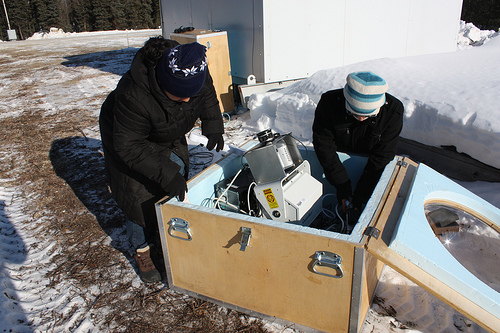
\includegraphics[width=0.9\linewidth]{gfx/HST1}
	\caption{HiST1 camera installation at the MF radar site in non-climate controlled box.}
	\label{fig:hst2}
\end{figure}
The blue insulation in this box was a help at night but a hindrance during the day, when temperatures rose to the order of $50^\circ$C.
This result led to detailed thermodynamic modeling for the climate control and cabinet system design for HiST Phase 2, as shown in Figure~\ref{fig:hist2cab}.
\begin{figure}
	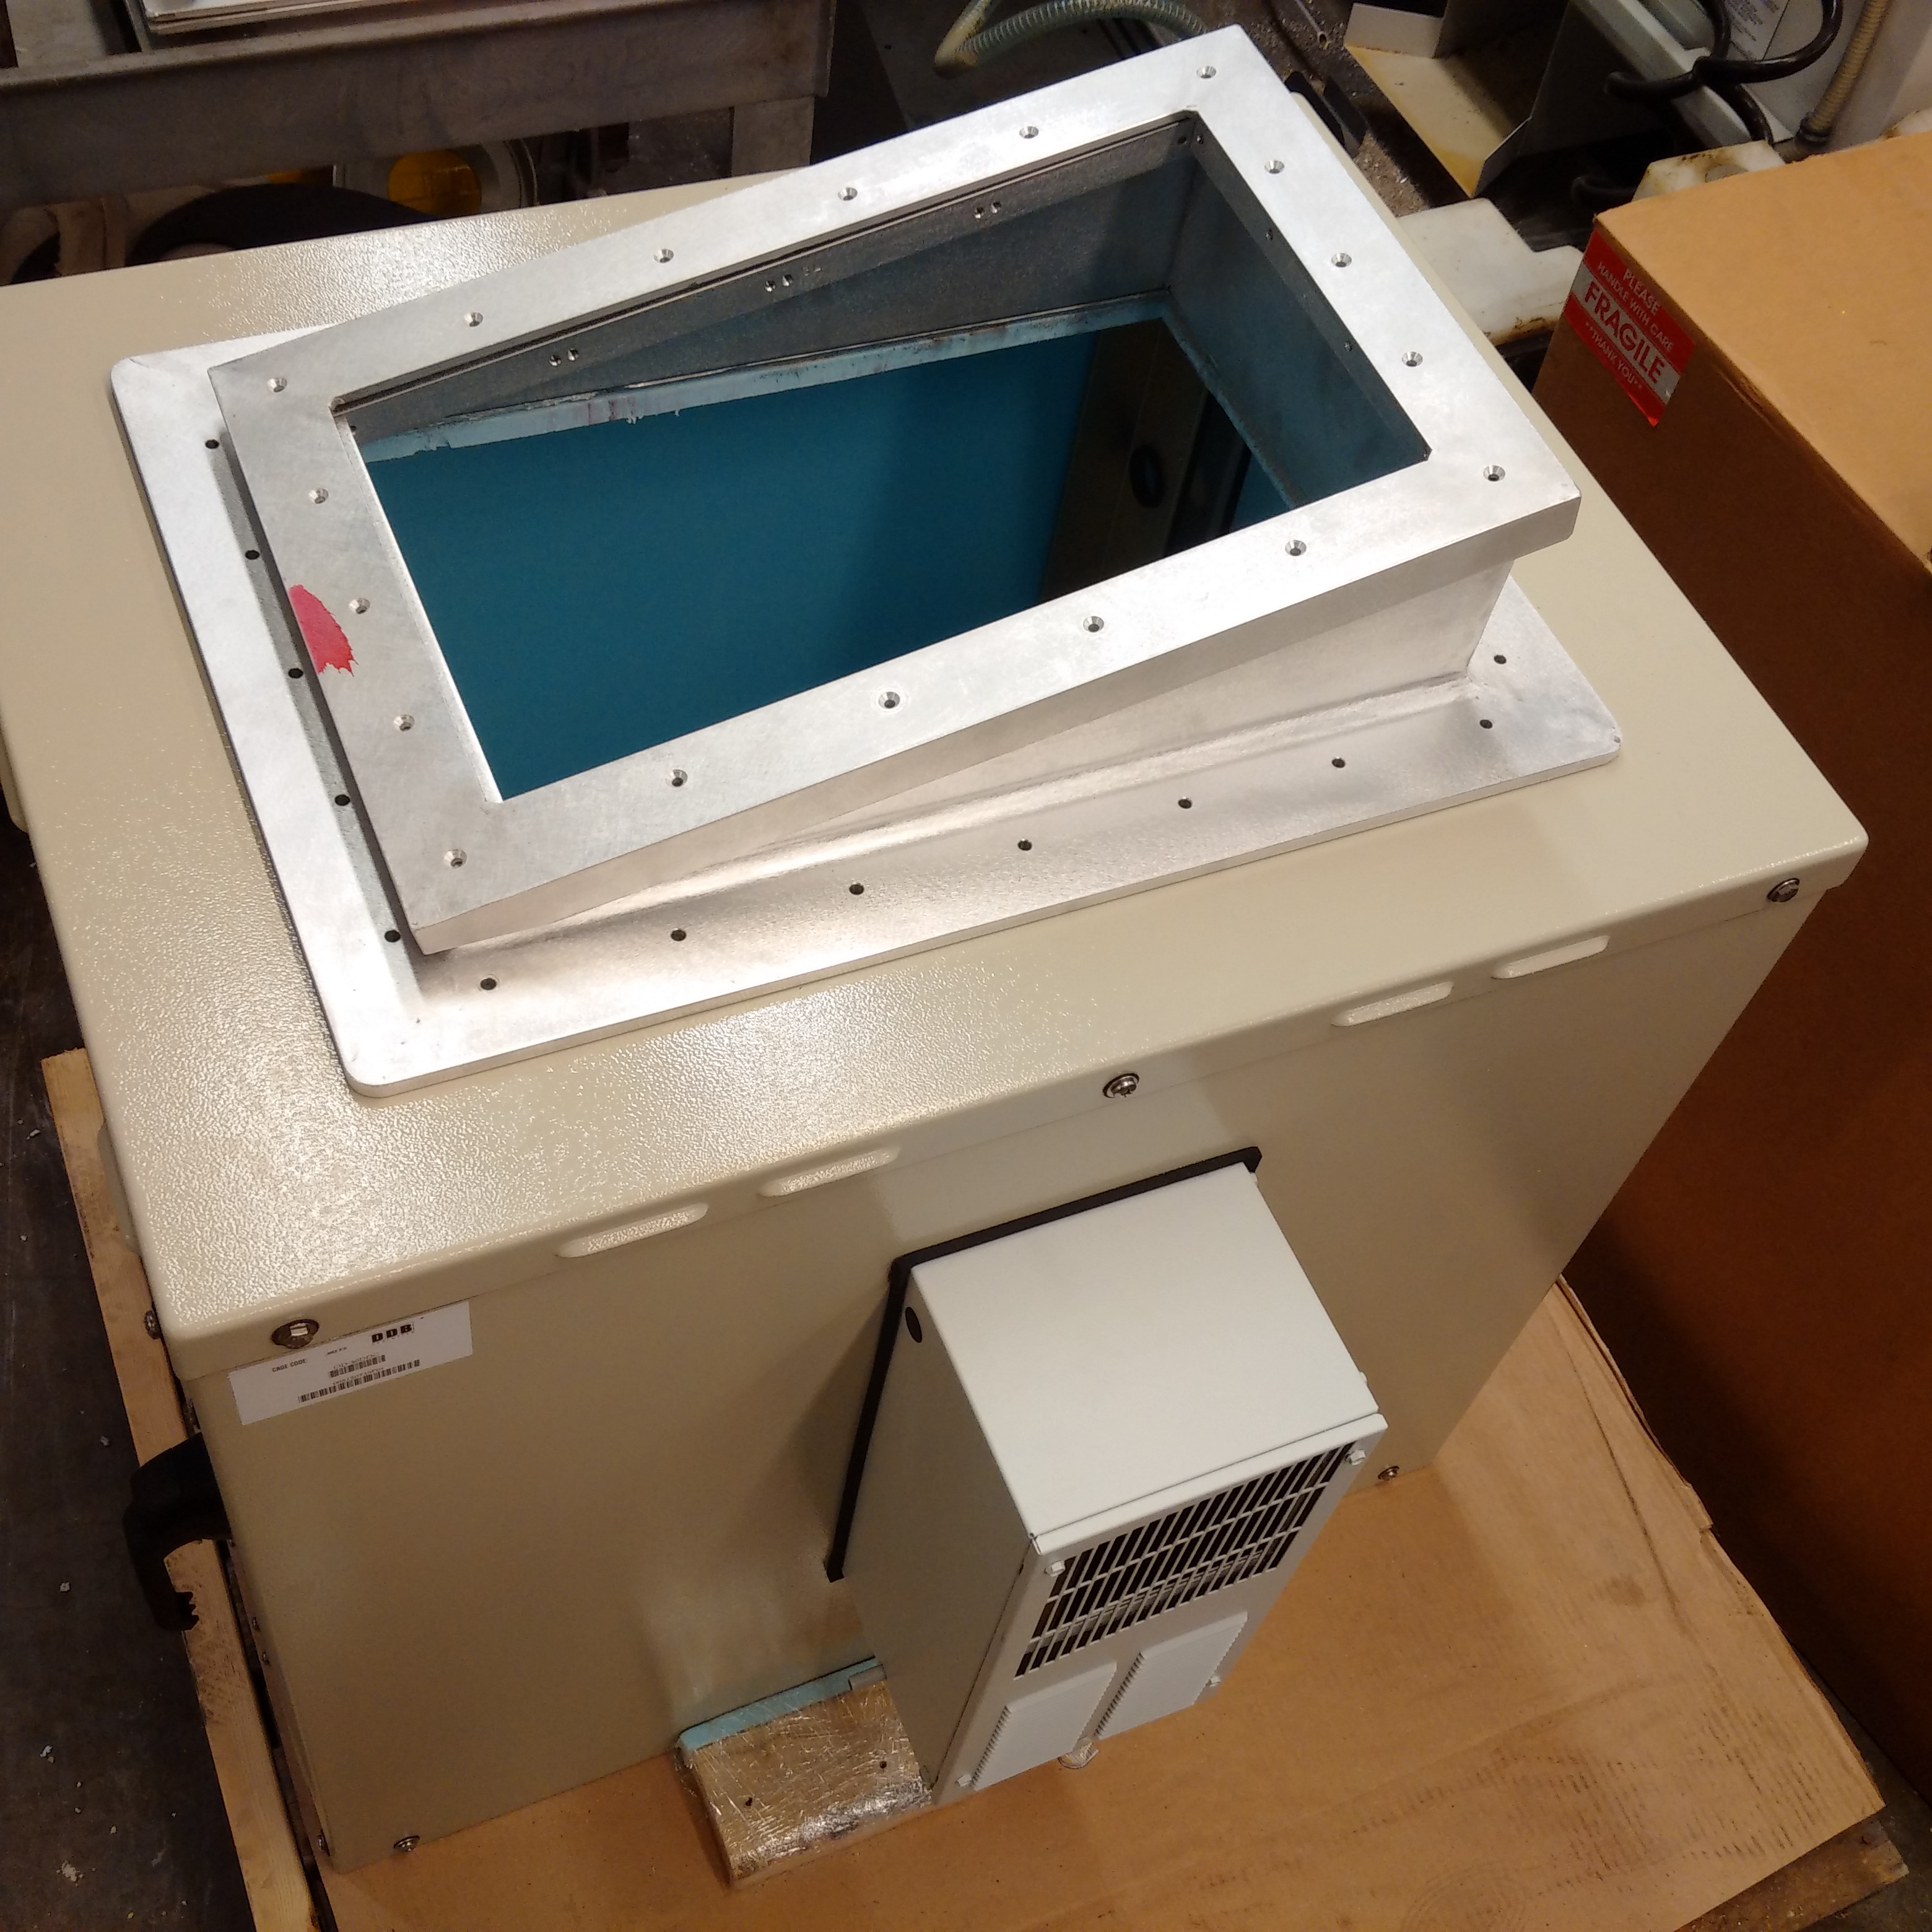
\includegraphics[width=\linewidth]{gfx/phase2cabinet}
	\caption{HiST Phase 2 cabinet with air conditioning as built in BU SIF.}
	\label{fig:hist2cab}
\end{figure}
This cabinet accommodates two cameras plus GPS and beacon receivers for enhanced data inversion via additional data inputs.
The next section describes the concerns involved with collecting and managing data from three to six cameras at remote unattended installations.

\FloatBarrier
\subsection{HiST Data}
A single camera in the HiST system collects over \unit[100]{GB} per hour, and given the remote unattended deployment of the cameras, substantial data reduction is necessary to avoid on-site human operation.
This reduction algorithm is described in detail in chapter~\ref{chapter:discrim}.
The data surviving this decision is further delineated by passing through the data inversion described in section~\ref{sec:inv}.

When using multiple instruments together to draw observational-based conclusions about the physics expressed by the phenomenon of interest, it is essential to know at least the relative timing error of each instrument. 
The HiST system employs GPSDOs at each camera site to yield timing accuracy $\ll \unit[1]{ms}$. 
Since this is a custom timing system, it is possible that errors in system design or equipment malfunction could cause an unexpected timing error. 
A convenient high temporal resolution test source in the common optical view are low earth orbit (LEO) satellites. 
LEO satellites are also easily visible with ISR in most modes of operation as bright targets > 10 times background.
Thus a tractable time verification can be achieved via an independent source--a geoscience instance of ``trust but verify''.
In particular, the Iridium constellation is a convenient candidate for time synchronization verification due to the large optical cross section and low orbit yielding an optically bright, fast-moving target. 
We must consider errors in SGP4 position propagation and ECI to azimuth and elevation (az/el) coördinate conversion.

The HiST geoscience optical instrument uses cameras including the Andor iXon 897 and iXon 888, with notional parameters described in Table~\ref{tab:ixonrate}. 
\begin{table}\centering
    \caption{Typical dataflow rates for high-speed auroral cameras.}\label{tab:ixonrate}
    \begin{tabular}{lllll}
        \toprule
        Camera & Resolution [pixels] & Bit depth [bits] & frame rate [Hz] & MB/sec \\
        \midrule
        iXon 897 & 512 x 512 & 16 & 50 & 26.2 \\
        iXon 887 & 512 x 512 & 14 & 30 & 15.7 \\
        \bottomrule
    \end{tabular}
\end{table}
It is important for experiment designers to note that camera datasheet frame rates are specified using conditions that are often unrealistic for the extended (many hours) observations typical in auroral observatories. 
By experiments in our lab, a derating of 5\% to 10\% is common for the Andor sCMOS and EMCCD cameras tested, with example sCMOS results shown in Table~\ref{tab:neomax}.
Even at the reduced frame rates in Table~\ref{tab:ixonrate}, imperfections in camera operations (e.g. dropped frames) were commonly observed, as often as multiple times per night.


A hardware monitor of the camera frame acquisition output accounts for any firmware glitches with regard to timing.
The deterministic counter in HiST shown in Figure~\ref{fig:histtime} uses the National Instruments PCIe-6321 with eight timers on an Application Specific Integrated Circuit (ASIC).
\begin{sidewaysfigure}\centering
    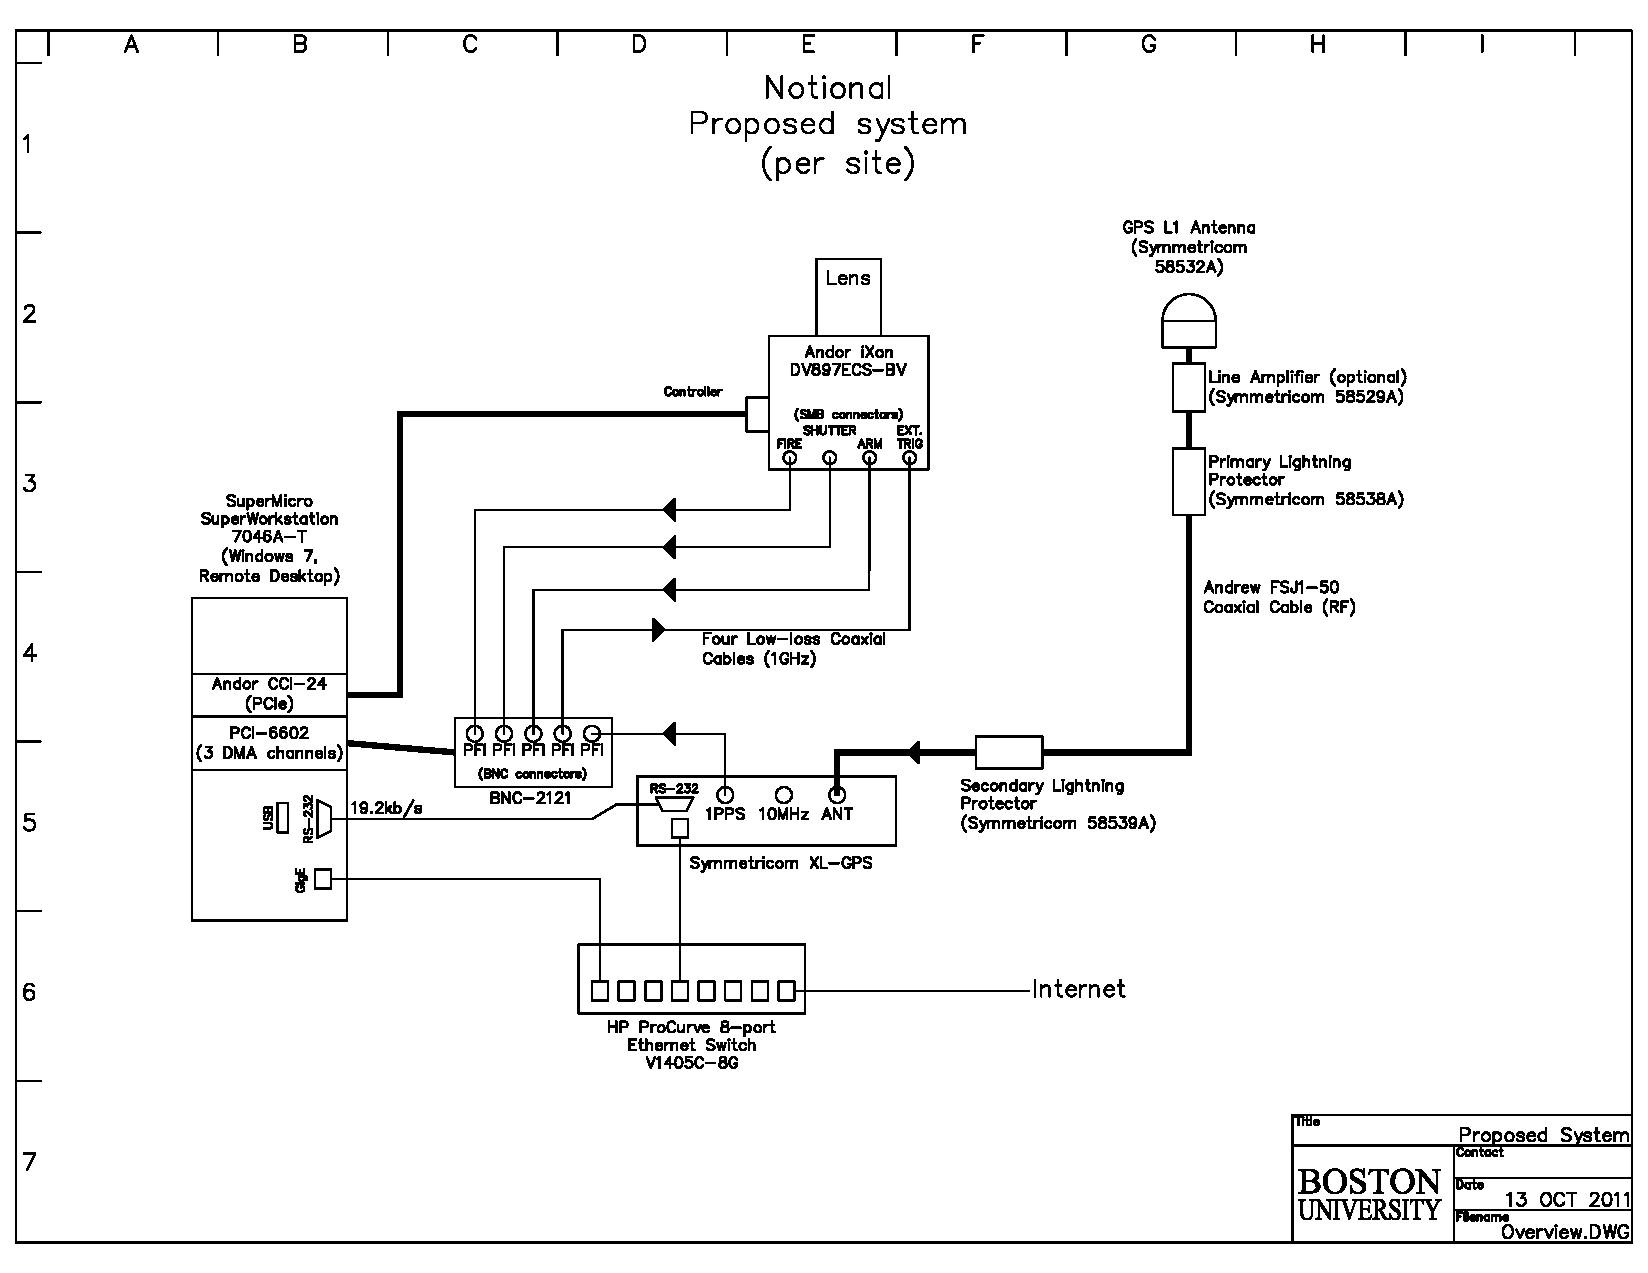
\includegraphics[page=1,width=0.95\linewidth]{gfx/ProposedTimingSystem}
    \caption{HiST timing system block diagram.}\label{fig:histtime}
\end{sidewaysfigure}
At the user's option, an additional deterministic timer per site is used to fire the cameras at precise intervals.
For simplicity and especially where the cameras are operated at distinct frame rates with a non-multiple relationship between the cameras, the cameras can be set to free run mode where the absolute time is recovered from the frame acquisition output.
In this manner, any camera with a frame acquisition binary output can be part of the HiST network.
Most scientific cameras with sufficient sensitivity have such an output.

The image collection software and hardware techniques developed in this dissertation are generalizable to any remote imaging system, and were used in developing the HiST Phase 2 instrument.
A map of candidate HiST Phase 2 sites (there will be three sites) is shown in Figure~\ref{fig:hist3}.
\begin{figure}
	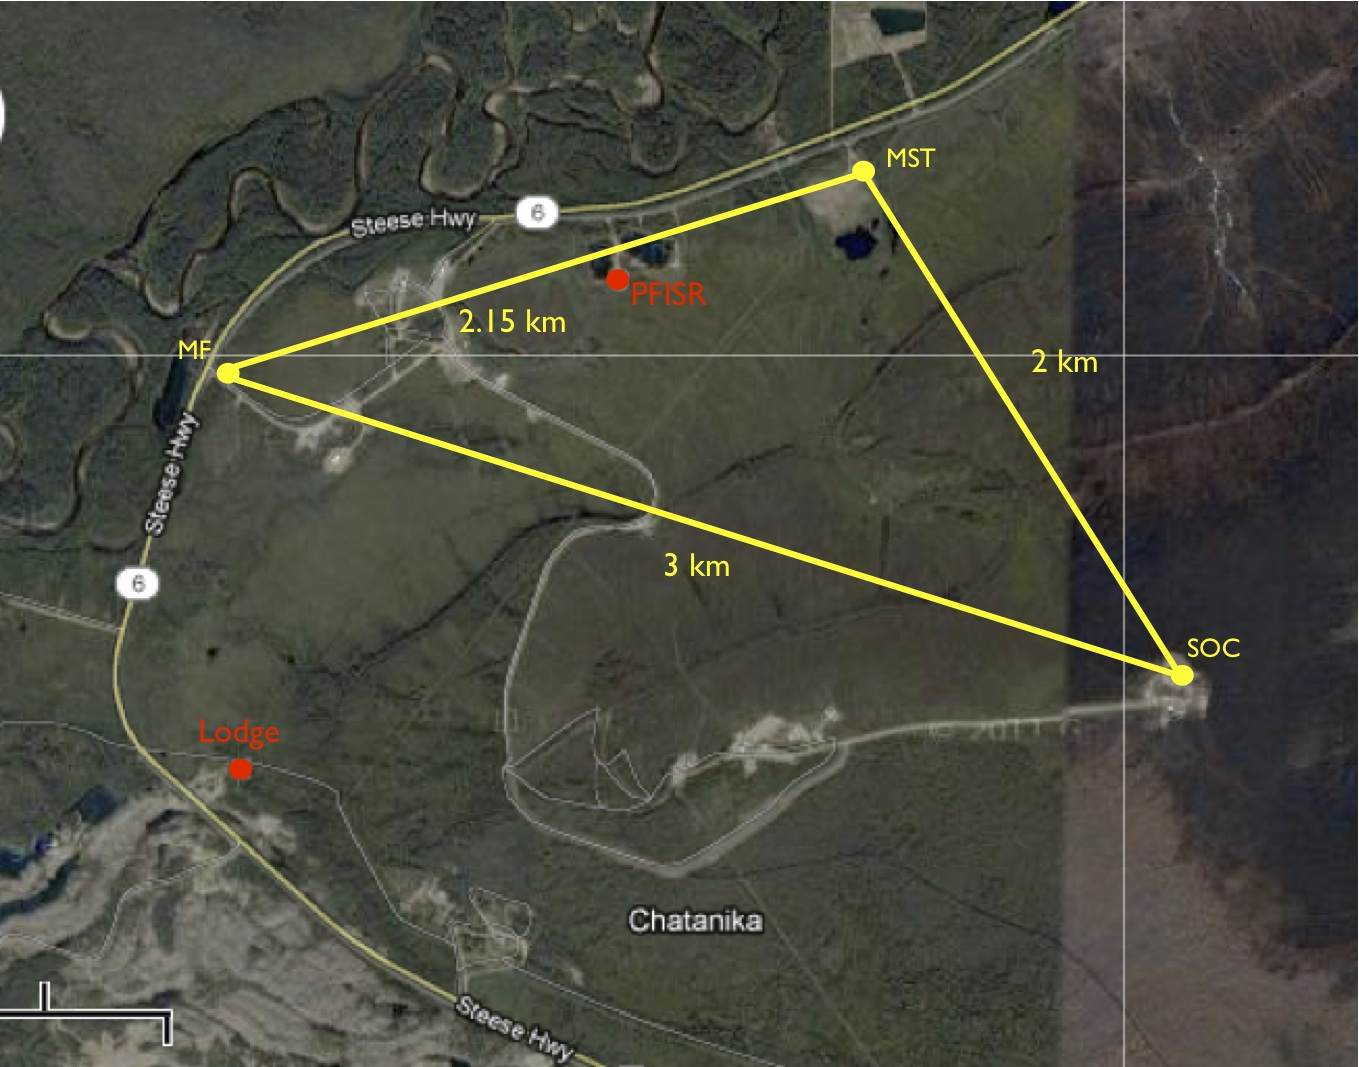
\includegraphics[width=\linewidth]{gfx/Optical_Sites3}
	\caption{Candidate sites for three site HiST Phase 2 deployment.}
	\label{fig:hist3}
\end{figure}
Initial processing will be with pairs of cameras, with the eventual goal of integrated three camera plus ISR data inversion.

